Para reduzir significativamente a dimensão dos mapas de características, eventualmente, após a camada convolucional, é utilizada uma camada chamada \textit{pooling}. A camada de \textit{pooling} divide o mapa de características de entrada em blocos de tamanhos iguais e processa cada bloco para criar um mapa de características condensado. O processamento dos blocos é definido por uma função de \textit{pool} que pode ser, por exemplo, a função máxima. Assim como na camada de convolução, na camada de \textit{pooling} também é preciso especificar o tamanho da região de \textit{pooling} e o \textit{stride} $s$ da operação, conforme exemplificado na Figura \ref{img:pooling} em que a região possui tamanho 2 x 2 e o \textit{stride} $s=1$ \cite{ref:buduma,ref:khan}.

\begin{figure}[!ht]
	\centering
	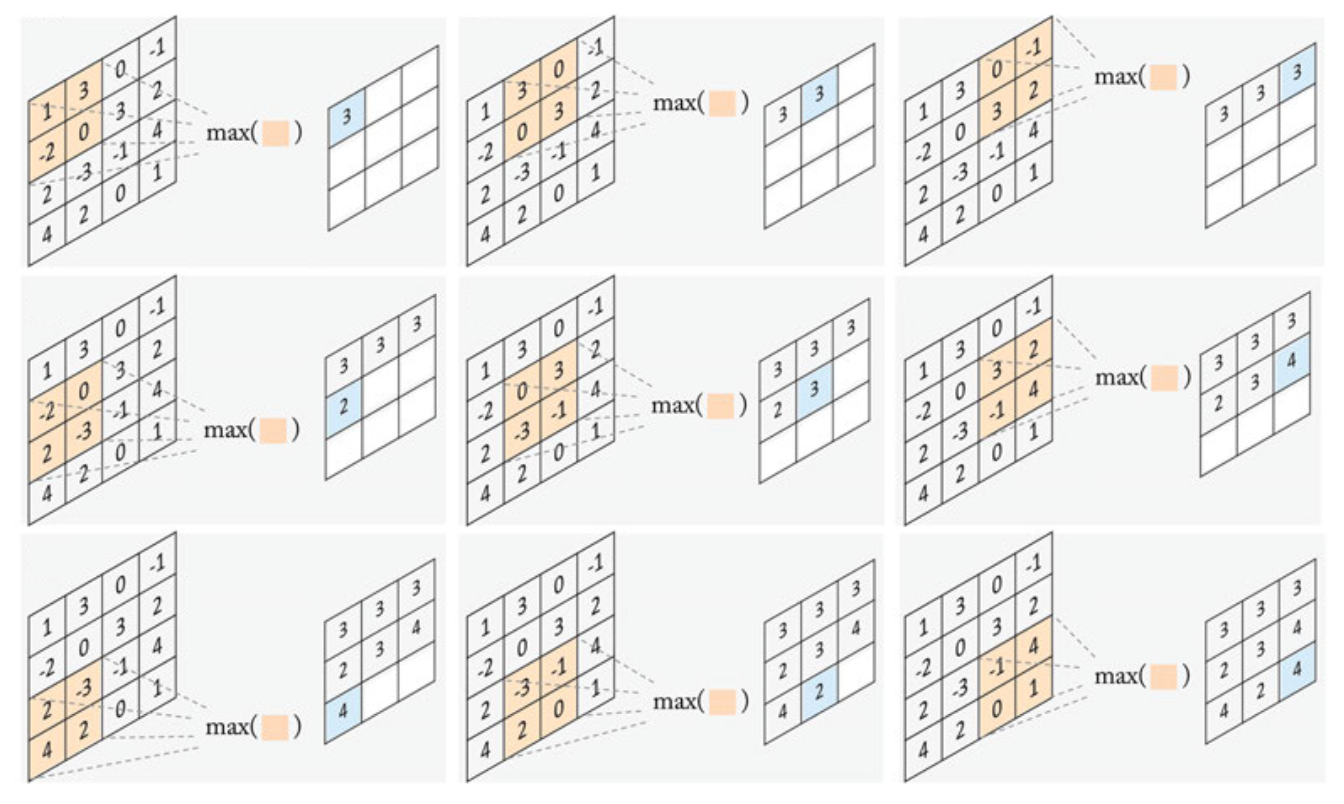
\includegraphics[width=0.9\textwidth]{./img/pooling}
	\caption{Exemplo de um processo de \textit{pooling} aplicado em uma entrada de tamanho 5 x 5 e uma região \textit{pooling} de tamanho 2 x 2. Fonte: \cite{ref:khan}.}
	\label{img:pooling}
\end{figure}

As últimas camadas de uma CNN normalmente são as \textit{Fully Connected Layers} (FCL), ou camadas completamente conectadas, as quais correspondem essencialmente às camadas de convolução que utilizam filtros de tamanho 1 x 1 em que cada elemento é densamente conectado à todos os elementos da camada anterior \cite{ref:khan}. Nesta última camada, adota-se tipicamente o uso da função \textit{Softmax}, também chamada de função exponencialmente normalizada, a qual escala o vetor de saída de forma que seus elementos pertençam a m intervalo entre $0$ e $1$ e que quando somados sejam igual a 1  \cite{ref:JAI-2017}. O processo de aprendizagem utilizado pelas FCL é baseado nos conceitos das RNAs do tipo MLP e no algoritmo de treinamento \textit{backpropagation} \cite{ref:gulli, ref:khan}.

Durante o processo de treinamento, as CNNs utilizam algumas técnicas para tentar evitar possíveis problemas, como \emph{overfiting}. Qualquer modificação feita em um algoritmo de AM com o objetivo de reduzir os erros de generalização é chamada de regularização \cite{ref:goodfellow}. Uma das abordagens mais populares utilizadas pelas CNNs para regularização é a técnica de \emph{Dropout}, a qual utiliza uma probabilidade $p$ de ativação em cada neurônio durante o treinamento. Essa abordagem elimina temporariamente alguns neurônios e suas respectivas ligações de acordo com a probabilidade a qual normalmente é $p = 0.5$. A camada \textit{Dropout} de ativação de um CNN aumenta de forma significativa o desempenho da rede para prever dados não vistos na fase de teste \cite{ref:khan}.
